% Template; to be used with:
%          spconf.sty  - ICASSP/ICIP LaTeX style file, and
%          IEEEbib.bst - IEEE bibliography style file.
% --------------------------------------------------------------------------
\documentclass{article}
\usepackage{spconf,amsmath,graphicx}

% Example definitions.
% --------------------
\def\x{{\mathbf x}}
\def\L{{\cal L}}

% Title.
% ------
\title{Graduate Certificate Intelligent Sensing Systems Practice Module Report Template}
%
% Single address.
% ---------------
\name{First1 Last1,  First2 Last2}
\address{Institute of Systems Science, National University of Singapore, Singapore 119615}

\begin{document}
%\ninept
%
\maketitle
%

\begin{abstract}

The abstract should consist of 1 paragraph describing the motivation for your report and a high-level explanation of the methodology you used and results obtained. Note: this project report template is modified from Stanford University CS230 report template https://cs230.stanford.edu/

\end{abstract}
%

\begin{keywords}
One, two, three, four,
\end{keywords}
%
\section{Introduction}
\label{sec:intro}

Explain the problem and why it is important. Discuss your motivation for pursuing this
problem. Give some background if necessary. Clearly state what the input and output
is. Be very explicit: “The input to our algorithm is an {image, video, RGB-D, audio}. We then use a {neural network, etc.} to output a predicted {age, facial expression, action music genre, etc.}.”

This is very important since different teams have different inputs/outputs spanning different
application domains. Being explicit about this makes it easier for readers.


\section{Literature review}
You should find existing references (e.g., papers, survey, industrial products), group them into categories based on their approaches, and discuss their strengths and weaknesses, as well as how they are similar to and differ from your work. In your opinion, which approaches were clever/good? What is the state-of-the-art?

\section{Dataset}
Describe your dataset: how many training/validation/test examples do you have? Is there
any pre-processing you did? What about normalization or data augmentation? What is the
resolution of your images? Include a citation on where you obtained your dataset from. Try to include examples of your data in the report (e.g. include an image, show a waveform, etc.).



\section{Proposed system}
Describe your proposed system. You might want to use a system architecture or flow chart to illustrate your proposed system. For each module, give a detailed description 
of how it works. Even you use pre-trained model in some modules, provide a description.

\section{Experimental results}

You should also give details about what (hyper)parameters you chose and how
you chose them. What your primary metrics are: accuracy, precision, etc. Provide equations for the metrics if necessary. You also need to evaluate your approach in various experimental setups. For results, you want to have a mixture of tables and plots. To reiterate, you must have both quantitative and qualitative results! Include visualizations of results, examples of where your approach failed and a discussion of why certain approach failed or succeeded. 

Some Latex examples are provided as follows. An inline equation is $a+b=c$. An example of one-column figure is provided in Figure \ref{figure1}.

\begin{equation}\label{equation block model}
B_{r,c}=\sum\{f(i,j)|(i,j)\in \Omega_{r,c}\}.
\end{equation}
\begin{equation}\label{equation 1}
\sum_{x}=a+b+\hat{c},
\end{equation}

\begin{figure}[tbh]
    \centerline{\begin{tabular}{cc|c}
        
\includegraphics[width=3cm]{iss.png}
        &
\includegraphics[width=3cm]{iss.png}& text\\
    (a) & (b) & (c)
    \end{tabular}}
    \caption{Test figure (single column).\label{figure1}}
\end{figure}

\begin{table}[tbh]
\caption{The performance comparison.}\label{table1} \centerline{
    \begin{tabular}{clc|r}
    \hline\hline
    Approach & Ref. \cite{He:16CVPR} & Ref. \cite{Nguyen:18IET} & Proposed approach\\
    Metric A & $0.8181$ & $0.9171$ & $0.9616$ \\\hline
    Metric B & $0.8236$ & $0.7654$ & $0.8615$ \\\hline
    \end{tabular}
    }
\end{table}

\subsection{DeeplabV3 Model Evaluation}
trained DeeplabV3 with cityscapes dataset on resnet v2 
but we were not able to complete due to low computation power.
\begin{table}[tbh]
\caption{The (hyper)parameters}\label{table2} \centerline{
    \begin{tabular}{clc}
    \hline\hline
    train epochs & 26 \\\hline
    batch size & 10 \\\hline
    decay & 2e-4 \\\hline
    max iteration & 30000 \\\hline
    initial learning rate & 7e-3 \\\hline
    \end{tabular}
    }
\end{table}

\begin{figure}[tbh]
    \centerline{\begin{tabular}{cc}
        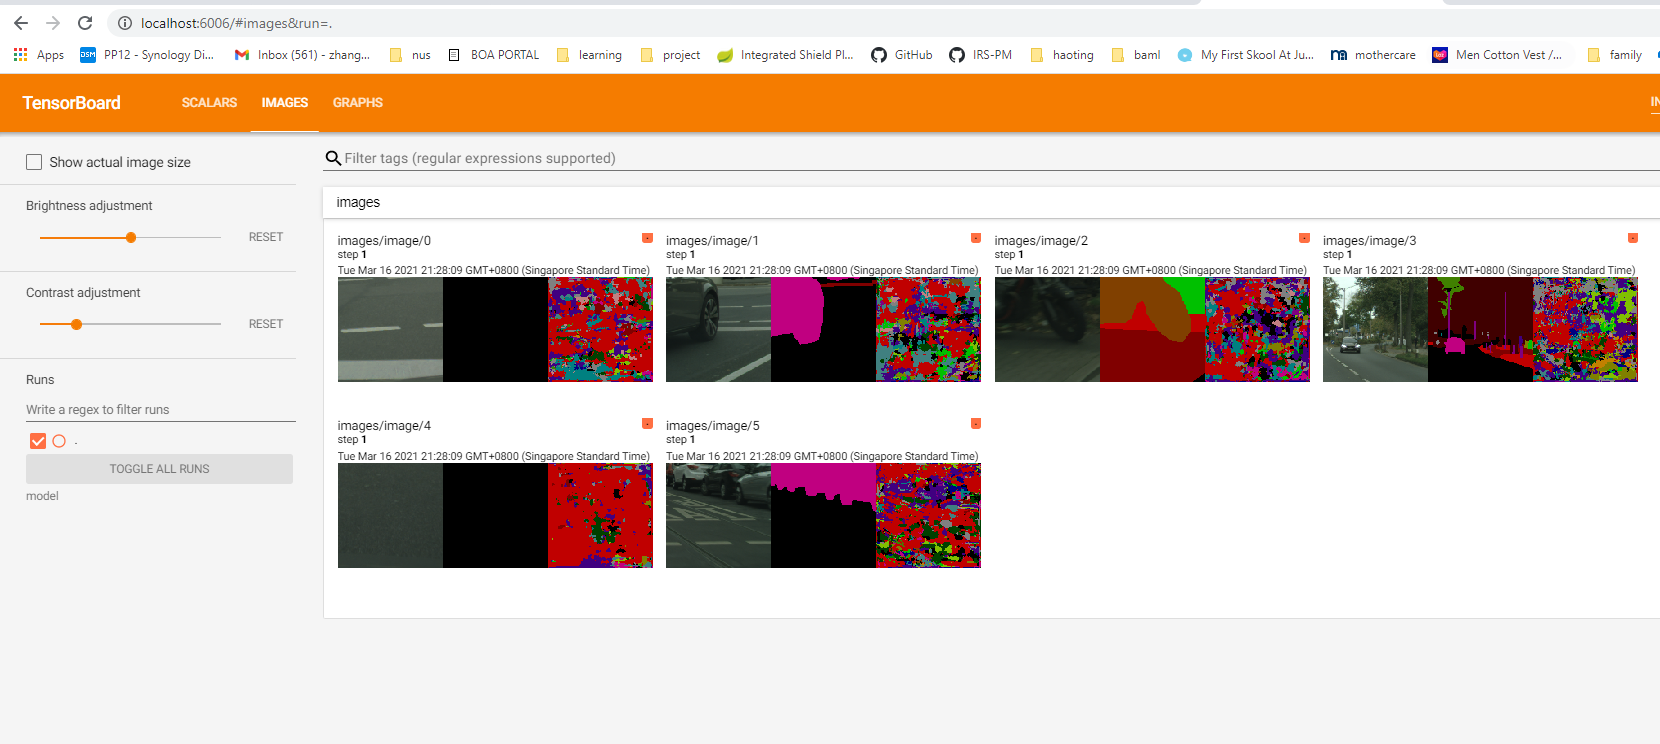
\includegraphics[width=8cm]{resnet_V2_101.png}\\
    (a)
    \end{tabular}}
    \caption{deeplabV3 on cityscapes dataset \label{figure2}}
\end{figure}

\subsection{Approach 1: Unet segmentation with MobileNetV2}

\begin{table}[tbh]
\caption{The (hyper)parameters}\label{table3} \centerline{
    \begin{tabular}{clc}
    \hline\hline
    train epochs & 36 \\\hline
    batch size & 8 \\\hline
    decay & 1e-4 \\\hline
    \end{tabular}
    }
\end{table}
Dice coefficient is used as loss function
\begin{equation}\label{equation 3}
Dice Loss=1-\frac{2\sum_{pixels}(y_{true}*y_{pred})}{\sum_{pixels}(y_{true})+\sum_{pixels}(y_{pred})}.
\end{equation}

\begin{figure}[tbh]
    \centerline{\begin{tabular}{cc}
        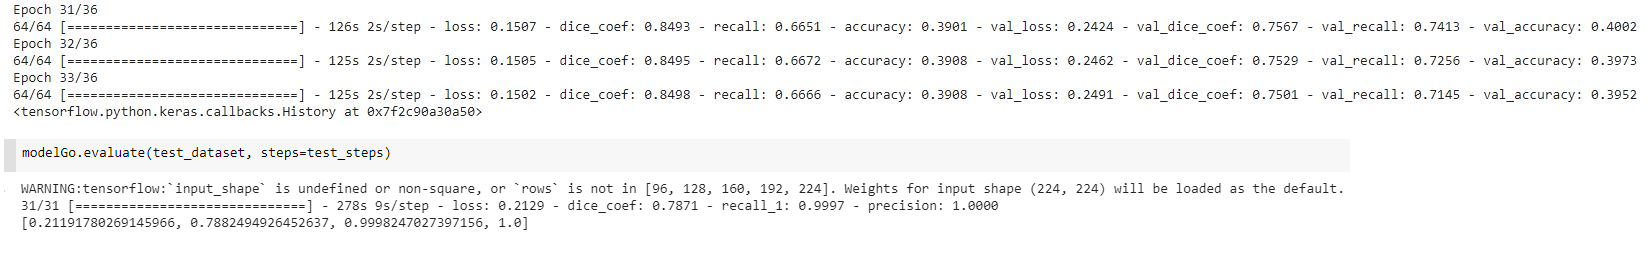
\includegraphics[width=4cm]{unet_grayscale_train_test.png}
        &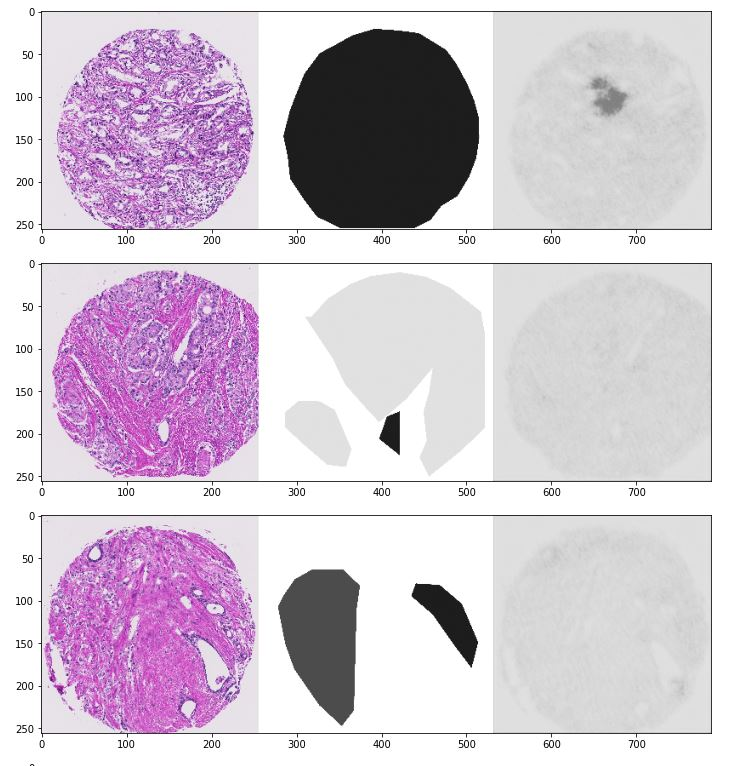
\includegraphics[width=4cm]{unet_grayscale.JPG}\\
    (a) & (b)
    \end{tabular}}
    \caption{Unet segmentation with MobileNetV2 \label{figure3}}
\end{figure}

\begin{table}[tbh]
\caption{The performance comparison.}\label{table4} \centerline{
    \begin{tabular}{clc}
    \hline\hline
    Approach & Dice coefficient\\
    Unet segmentation (Approach 1) & $0.7871$ \\\hline
    \end{tabular}
    }
\end{table}


\subsection{Approach 2: Unet segmentation with Patch Pre-processing}
\begin{table}[tbh]
\caption{The (hyper)parameters}\label{table5} \centerline{
    \begin{tabular}{clc}
    \hline\hline
    train epochs & 16 \\\hline
    batch size & 32 \\\hline
    decay & 1e-4 \\\hline
    \end{tabular}
    }
\end{table}
Dice coefficient is used as loss function and is provided in Equation \eqref{equation 3}
\begin{figure}[tbh]
    \centerline{\begin{tabular}{cc}
        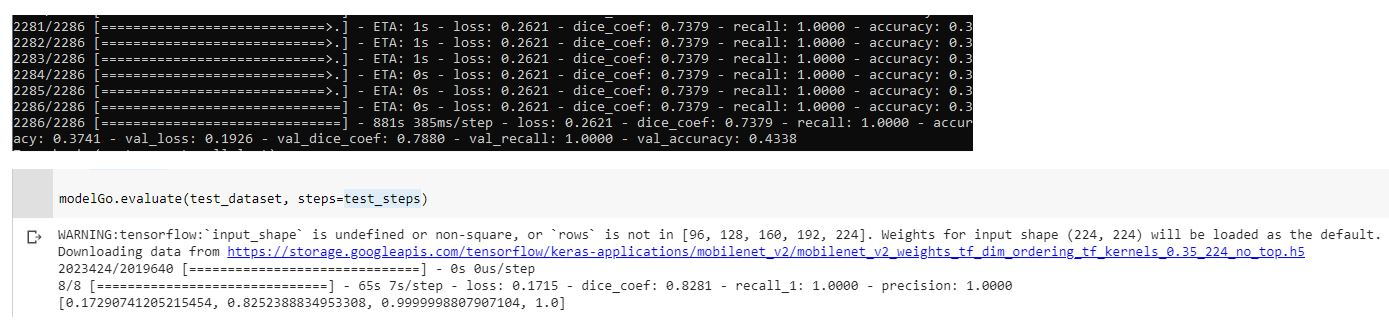
\includegraphics[width=4cm]{unet_patch_train_test.JPG}
        &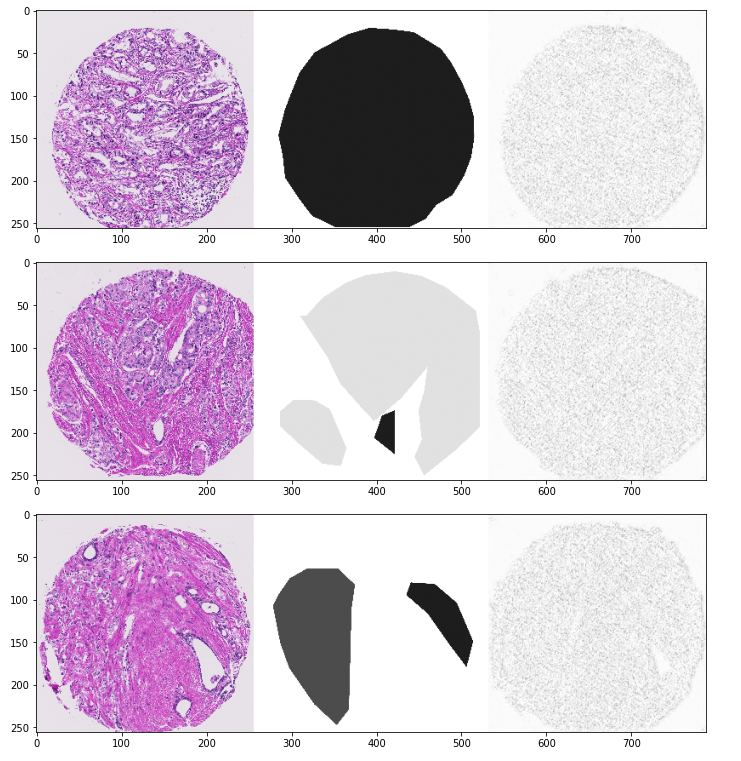
\includegraphics[width=4cm]{unet_patch.png}\\
    (a) & (b)
    \end{tabular}}
    \caption{Unet patch \label{figure4}}
\end{figure}

\begin{table}[tbh]
\caption{The performance comparison.}\label{table6} \centerline{
    \begin{tabular}{clc}
    \hline\hline
    Approach & Dice coefficient\\
    Unet segmentation (Approach 1) & $0.7871$ \\\hline
    Unet patch (Approach 2) & $0.8281$ \\\hline
    \end{tabular}
    }
\end{table}

\subsection{Approach 3: Unet segmentation by Increasing EPOCH}
\begin{table}[tbh]
\caption{The (hyper)parameters}\label{table7} \centerline{
    \begin{tabular}{clc}
    \hline\hline
    train epochs & 100 \\\hline
    batch size & 8 \\\hline
    decay & 1e-4 \\\hline
    \end{tabular}
    }
\end{table}
Dice coefficient is used as loss function and is provided in Equation \eqref{equation 3}
\begin{figure}[tbh]
    \centerline{\begin{tabular}{cc}
        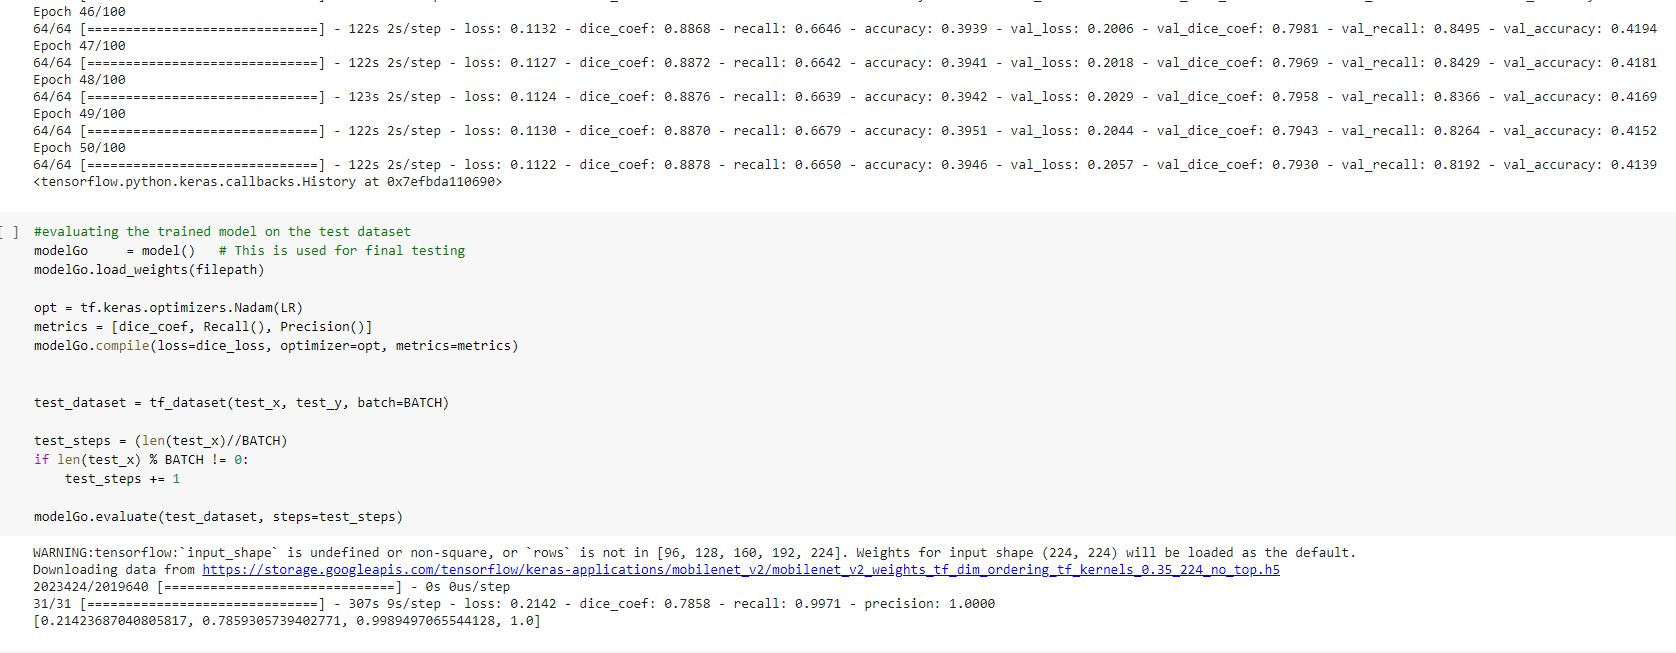
\includegraphics[width=4cm]{unet_increase_epoch_train_test.JPG}
        &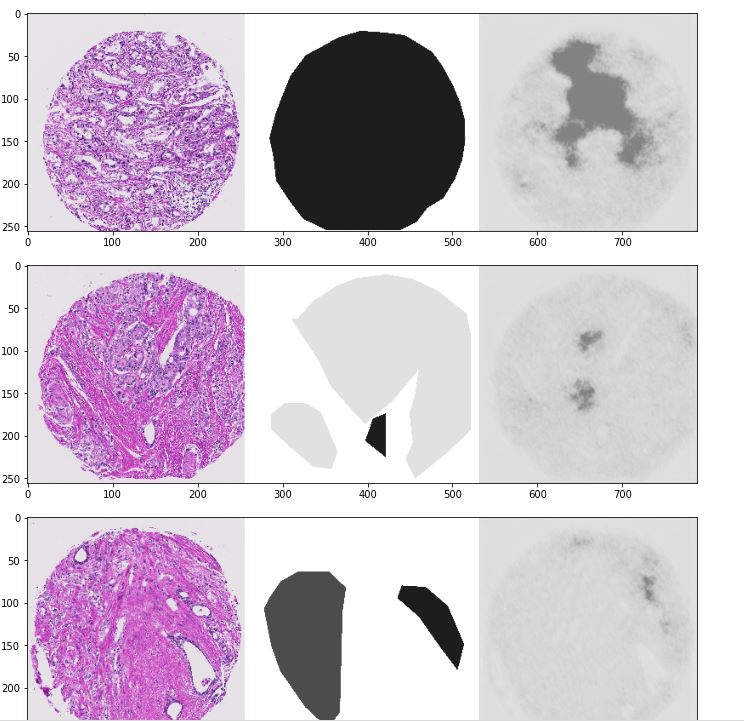
\includegraphics[width=4cm]{unet_increase_epoch.JPG}\\
    (a) & (b)
    \end{tabular}}
    \caption{Unet with increased EPOCH \label{figure5}}
\end{figure}

\begin{table}[tbh]
\caption{The performance comparison.}\label{table8} \centerline{
    \begin{tabular}{clc}
    \hline\hline
    Approach & Dice coefficient\\
    Unet segmentation (Approach 1) & $0.7871$ \\\hline
    Unet patch (Approach 2) & $0.8281$ \\\hline
    Unet increased EPOCH (Approach 3) & $0.7858$ \\\hline
    \end{tabular}
    }
\end{table}

\subsection{Approach 4: Unet segmentation with HSV augmentation}
\begin{table}[tbh]
\caption{The (hyper)parameters}\label{table9} \centerline{
    \begin{tabular}{clc}
    \hline\hline
    train epochs & 36 \\\hline
    batch size & 8 \\\hline
    decay & 1e-4 \\\hline
    \end{tabular}
    }
\end{table}
Dice coefficient is used as loss function and is provided in Equation \eqref{equation 3}
\begin{figure}[tbh]
    \centerline{\begin{tabular}{cc}
        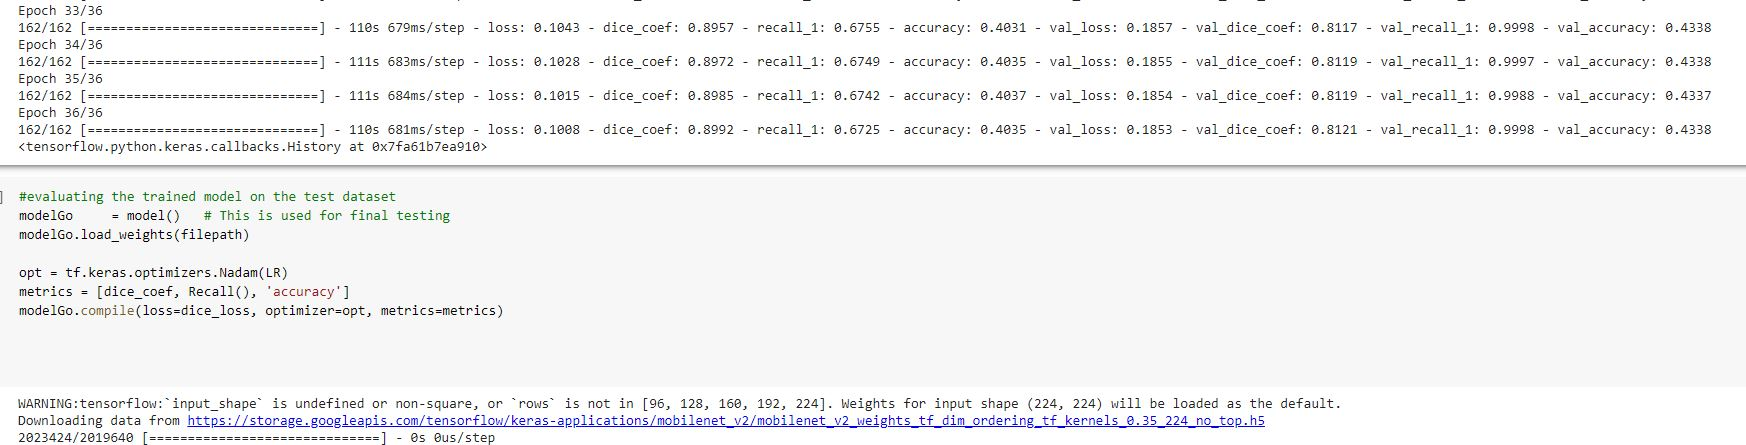
\includegraphics[width=4cm]{unet_hsv_train_test.JPG}
        &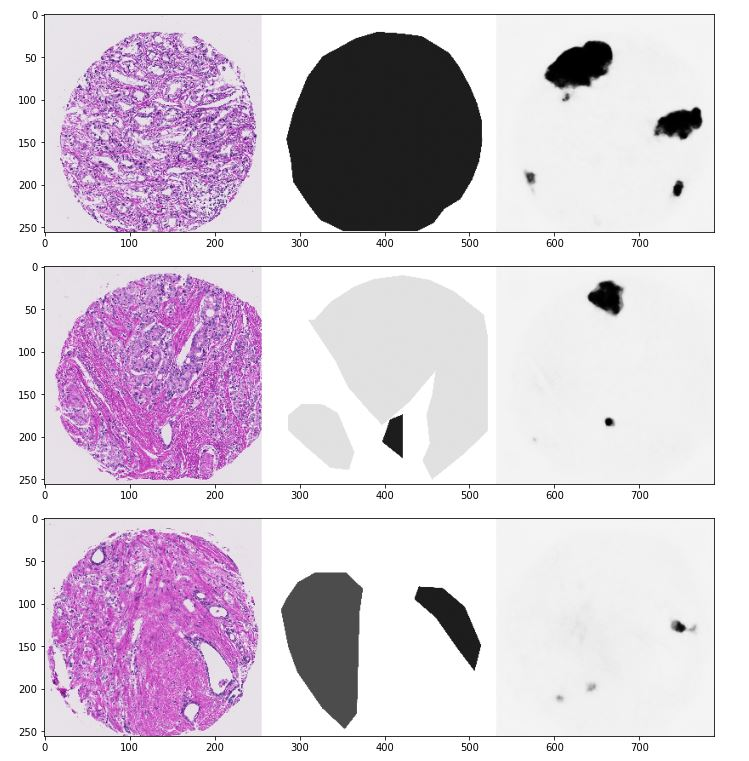
\includegraphics[width=4cm]{unet_hsv.JPG}\\
    (a) & (b)
    \end{tabular}}
    \caption{Unet hsv \label{figure6}}
\end{figure}

\begin{table}[tbh]
\caption{The performance comparison.}\label{table10} \centerline{
    \begin{tabular}{clc}
    \hline\hline
    Approach & Dice coefficient\\
    Unet segmentation (Approach 1) & $0.7871$ \\\hline
    Unet patch (Approach 2) & $0.8281$ \\\hline
    Unet increased EPOCH (Approach 3) & $0.7858$ \\\hline
    Unet hsv (Approach 4) & $0.8398$ \\\hline
    \end{tabular}
    }
\end{table}

\subsection{Approach 5: Unet segmentation with HED augmentation}
\begin{table}[tbh]
\caption{The (hyper)parameters}\label{table11} \centerline{
    \begin{tabular}{clc}
    \hline\hline
    train epochs & 36 \\\hline
    batch size & 8 \\\hline
    decay & 1e-4 \\\hline
    \end{tabular}
    }
\end{table}
Dice coefficient is used as loss function and is provided in Equation \eqref{equation 3}
\begin{figure}[tbh]
    \centerline{\begin{tabular}{cc}
        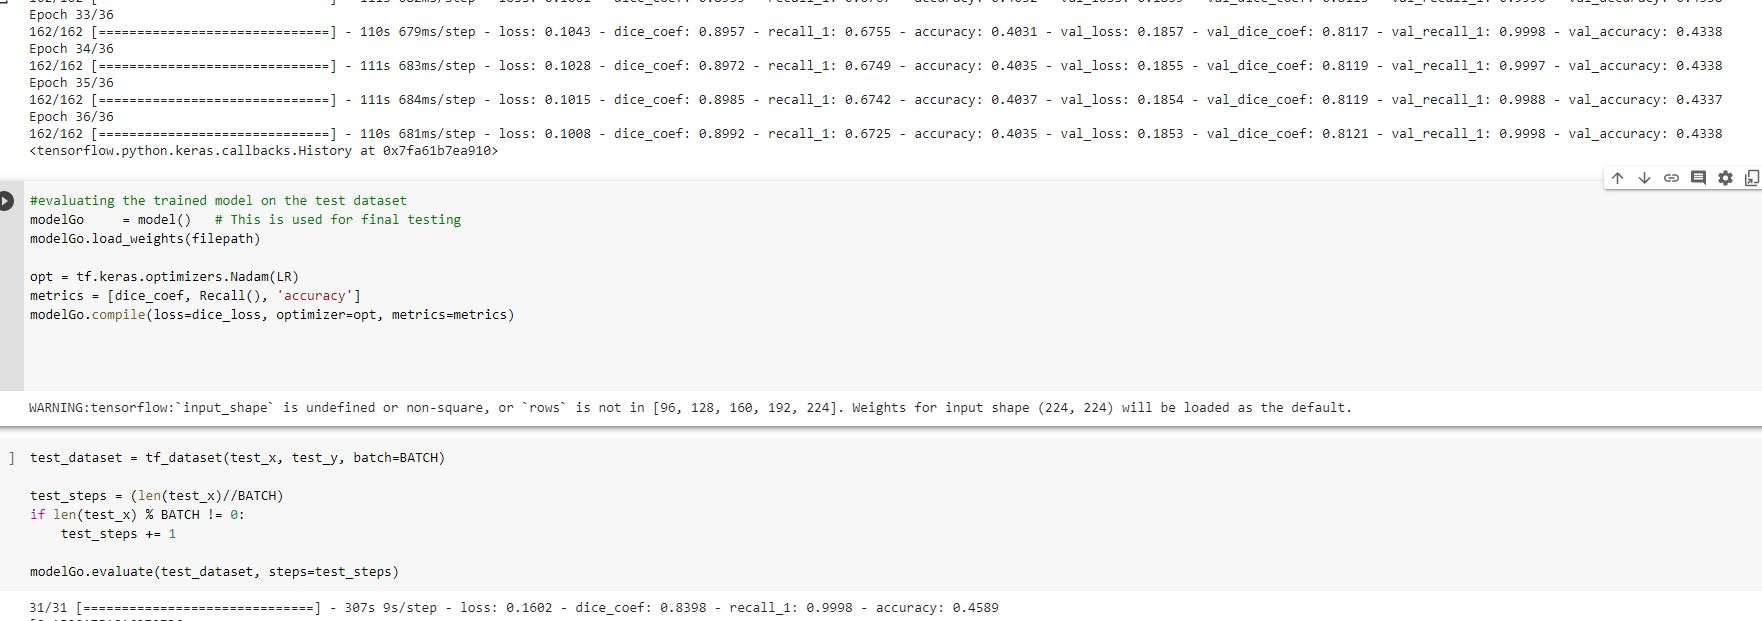
\includegraphics[width=4cm]{unet_hed_train_test.JPG}
        &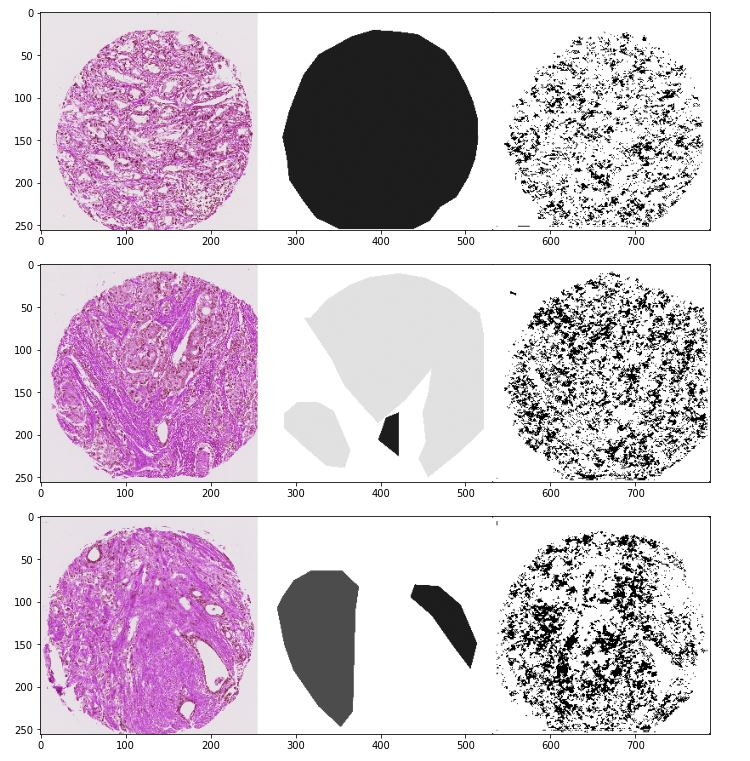
\includegraphics[width=4cm]{unet_hed.JPG}\\
    (a) & (b)
    \end{tabular}}
    \caption{Unet hed \label{figure7}}
\end{figure}

\begin{table}[tbh]
\caption{The performance comparison.}\label{table12} \centerline{
    \begin{tabular}{clc}
    \hline\hline
    Approach & Dice coefficient\\
    Unet segmentation (Approach 1) & $0.7871$ \\\hline
    Unet patch (Approach 2) & $0.8281$ \\\hline
    Unet increased EPOCH (Approach 3) & $0.7858$ \\\hline
    Unet hsv (Approach 4) & $0.8398$ \\\hline
    Unet hed (Approach 5) & $0.8398$ \\\hline
    \end{tabular}
    }
\end{table}

\subsection{Approach 6: Unet segmentation with }
\begin{table}[tbh]
\caption{The (hyper)parameters}\label{table11} \centerline{
    \begin{tabular}{clc}
    \hline\hline
    train epochs & 36 \\\hline
    batch size & 8 \\\hline
    decay & 1e-4 \\\hline
    \end{tabular}
    }
\end{table}
Dice coefficient is used as loss function and is provided in Equation \eqref{equation 3}
\begin{figure}[tbh]
    \centerline{\begin{tabular}{cc}
        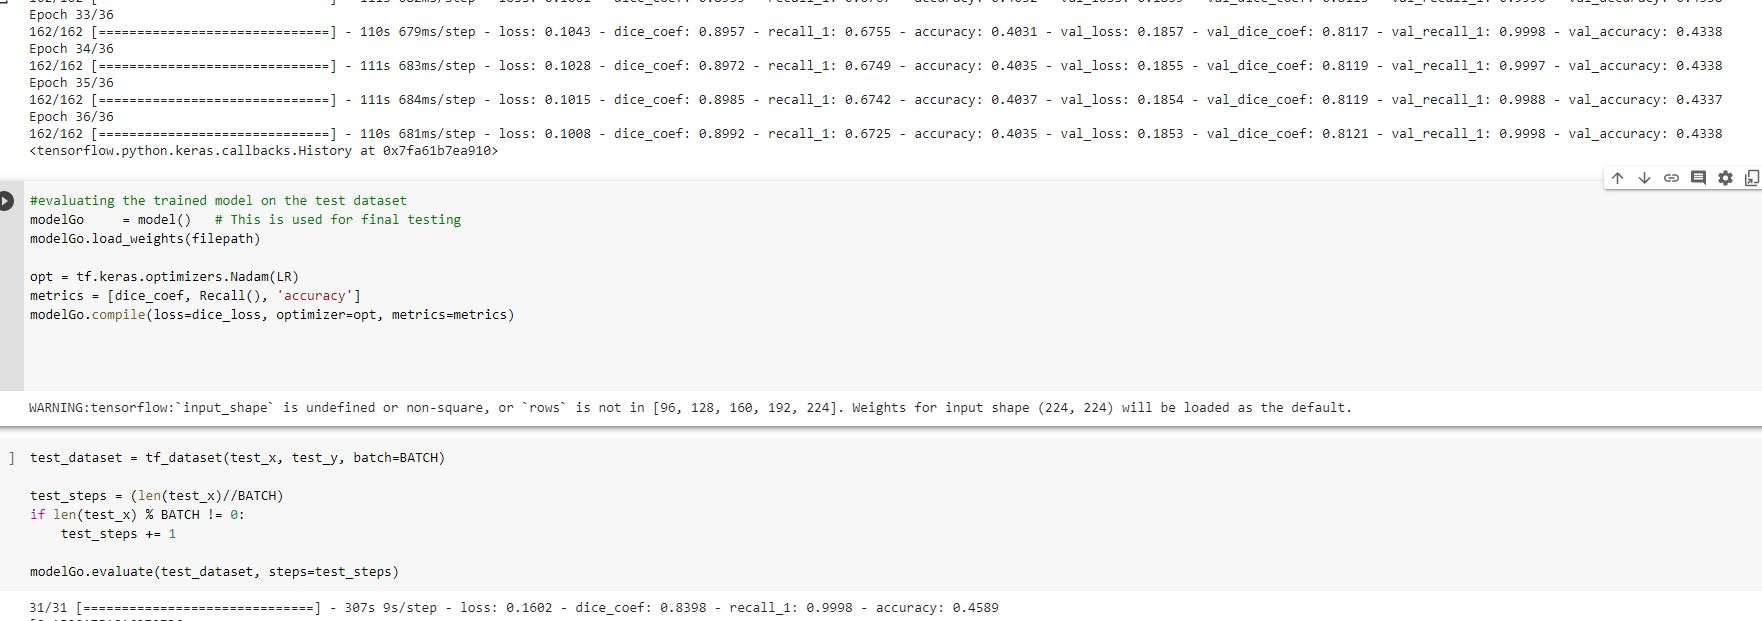
\includegraphics[width=4cm]{unet_hed_train_test.JPG}
        &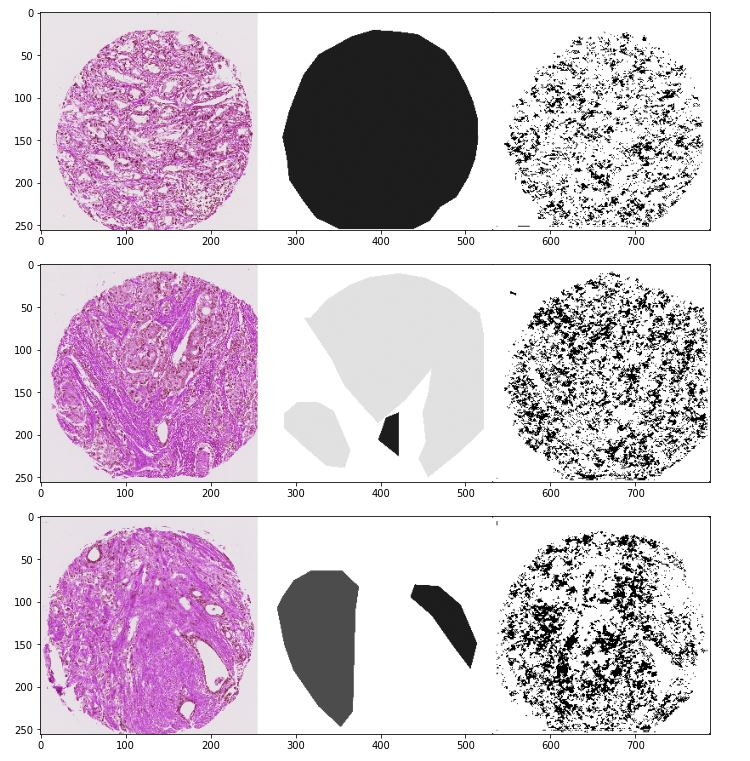
\includegraphics[width=4cm]{unet_hed.JPG}\\
    (a) & (b)
    \end{tabular}}
    \caption{Unet hed \label{figure7}}
\end{figure}

\begin{table}[tbh]
\caption{The performance comparison.}\label{table12} \centerline{
    \begin{tabular}{clc}
    \hline\hline
    Approach & Dice coefficient\\
    Unet segmentation (Approach 1) & $0.7871$ \\\hline
    Unet patch (Approach 2) & $0.8281$ \\\hline
    Unet increased EPOCH (Approach 3) & $0.7858$ \\\hline
    Unet hsv (Approach 4) & $0.8398$ \\\hline
    Unet hed (Approach 5) & $0.8398$ \\\hline
    \end{tabular}
    }
\end{table}

\section{Conclusions and future work}
Summarize your report and reiterate key points. Why do you think that some algorithms worked better than others? For future work, if you had more time, more team members, or more computational resources, what would you explore?

\section{Contributions}
This section should describe contributions of each team member to the project.

\bibliographystyle{IEEEbib}
\bibliography{references}

\end{document}
